\section{Introducción}

\begin{frame}
\frametitle{Motivación - ¿por qué NoSQL?}
\begin{itemize}

\item	El nombre NoSQL surge para denominar un conjunto de bases
	de datos recientemente desarrolladas que no siguen el modelo
	relacional (y por lo general no permiten consultas en SQL).
	Es a veces tomado como ``\textit{Not Only SQL}''.
	\pause

\item	La necesidad de alejarse del modelo relacional llega
	principalmente con los enormes volúmenes de datos de la web,
	para los cuales necesitamos escalar horizontalmente.
	\pause

\item	También, pueden adaptarse mejor al modelo de los datos y facilitar
	el desarrollo (ejemplo: BDOG). Según \textit{NoSQL Distilled} mucho
	tiempo del desarrollo de una aplicación es dedicado a mapear entre
	estructuras en memoria y la base de datos (comúnmente llamado
	``\textit{Impedance mismatch}'').
\end{itemize}
\end{frame}

\begin{frame}
\frametitle{Impedance mismatch}
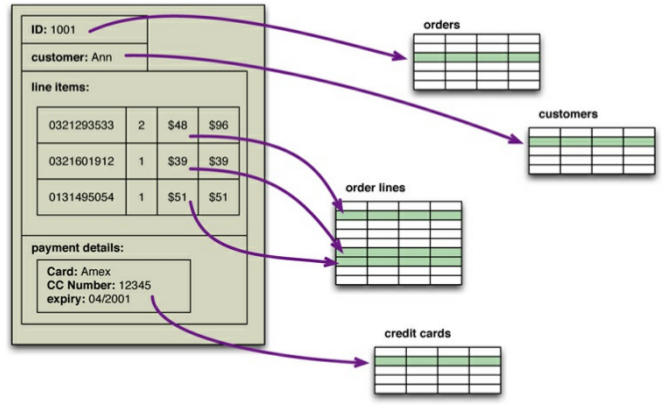
\includegraphics[width=\linewidth,height=\textheight,keepaspectratio]{impedance}
\end{frame}

\begin{frame}
\frametitle{Caracterización}
\begin{itemize}

\item	Si bien no hay una definición precisa de ``Base de datos
	NoSQL''. Suelen tener las siguientes características:
	\pause
	\begin{itemize}
	\item	No usan el modelo relacional.
		\pause

	\item	Pueden correr fácilmente en clusters (\textit{scale-out}
		vs. \textit{scale-up}) sin SPOFs (\textit{single point of
		failure}).
		\pause

	\item	Operan sin un esquema fijo, permitiendo agregar campos
		a los registros \textit{on-the-fly}.
		\pause

	\item	Usualmente son nuevas (posteriores al 2000) y software
		libre.
	\end{itemize}
	\pause

\item	No apuntan a ser un reemplazo de las bases de datos relacionales,
	pero dan otra opción a nuevos desarrollos. (Para datos no tan
	gigantescos, la mejora en rendimiento no es muy apreciable).
\end{itemize}
\end{frame}
